% F2: sectors of the field invariant s on the real slice E.B = 0 (3D, fixed perspective).
% Generated by scripts/F2_sectors.py -> figures/F2-sectors.pdf.  No data enter; the level c = 1 is a display choice.
\begin{figure}[t]
\centering
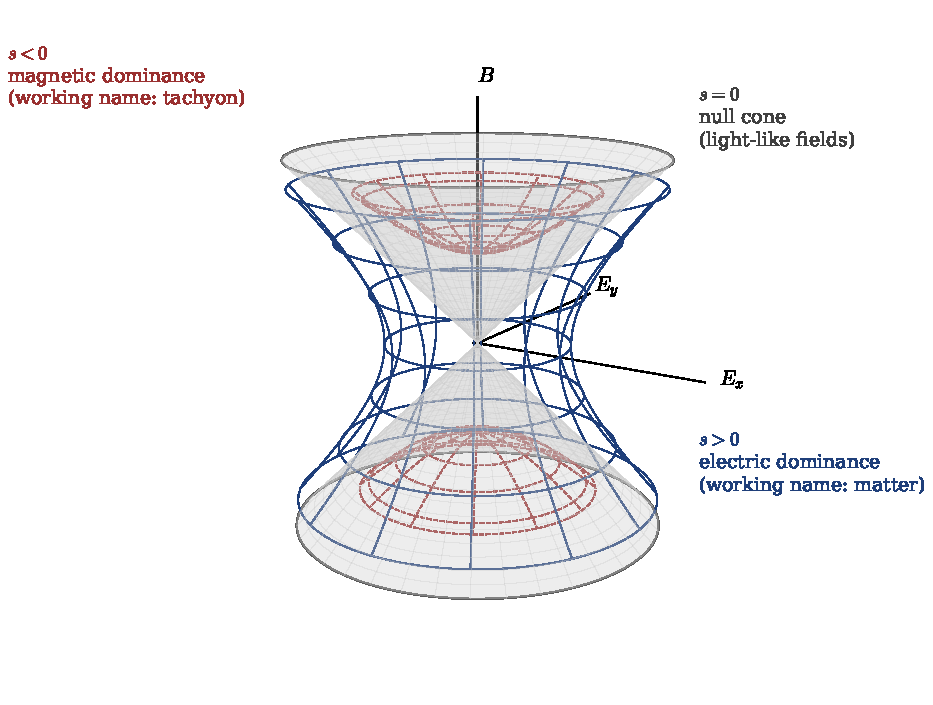
\includegraphics[width=0.78\textwidth]{figures/F2-sectors.pdf}
\caption{The three sectors of $s=z\cdot z$ on the slice where $\mathbf E\perp\mathbf B$, so that
$s=|\mathbf E|^2-|\mathbf B|^2$ is real ($\mathbf E$ horizontal, $\mathbf B$ vertical). Grey: the null cone
$s=0$ (light-like fields; the apex is the zero field). Solid: the level set $s=+1$ (electric dominance).
Dashed: the level set $s=-1$ (magnetic dominance). In the full space $\mathbb C^3$ the level sets
$s=c\neq0$ are the orbits of the Lorentz group $SO(3,\mathbb C)$, and the duality quarter turn
$z\mapsto iz$ maps the level $c$ to $-c$ (Proposition~\ref{prop:A-orbits}). The picture is a
three-dimensional slice of a six-dimensional space. \Established{} as geometry; the names matter and
tachyon are the working assignment of round v4.8.0-r07 and a \Reading.}
\label{fig:A-sectors}
\end{figure}
